\documentclass[10pt,a4paper,twocolumn]{article}
\usepackage[margin=19mm,top=22mm,bottom=22mm]{geometry}
\usepackage{fontspec}
\usepackage{kotex}
\setmainfont{NotoSansKR.ttf}[
  Path=fonts/,
  Renderer=Harfbuzz,
  UprightFeatures={RawFeature={axis={wght=400}}},
  BoldFont=NotoSansKR.ttf,
  BoldFeatures={RawFeature={axis={wght=700}}}
]
\setsansfont{NotoSansKR.ttf}[
  Path=fonts/,
  Renderer=Harfbuzz,
  UprightFeatures={RawFeature={axis={wght=400}}},
  BoldFont=NotoSansKR.ttf,
  BoldFeatures={RawFeature={axis={wght=700}}}
]
\usepackage{amsmath,amssymb,amsfonts}
\usepackage{graphicx}
\usepackage{array,booktabs,float,xcolor,url,microtype,balance,placeins}
\usepackage{fancyhdr,caption,siunitx}
\usepackage[hidelinks]{hyperref}
\hypersetup{pdftitle={모의 열 공정의 매개변수 불확실성에서 PID, LQR, LQI 제어기의 강인성과 성능 상충관계},pdfauthor={Mu-Won Lee},pdfsubject={제어기 비교 연구},pdfkeywords={PID, LQR, LQI, 열 공정, 매개변수 불확실성}}
\usepackage[nameinlink,noabbrev]{cleveref}
\usepackage[backend=biber,style=numeric-comp,sorting=none,maxbibnames=6]{biblatex}
\addbibresource{references.bib}
\captionsetup{font=small,labelfont=bf}
\renewcommand{\figurename}{그림}
\renewcommand{\tablename}{표}
\crefname{figure}{그림}{그림}
\crefname{table}{표}{표}
\AtBeginDocument{%
  \renewcommand{\crefpairconjunction}{ 및 }%
  \renewcommand{\crefmiddleconjunction}{, }%
  \renewcommand{\creflastconjunction}{ 및 }%
  \renewcommand{\crefpairgroupconjunction}{ 및 }%
  \renewcommand{\crefmiddlegroupconjunction}{, }%
  \renewcommand{\creflastgroupconjunction}{ 및 }%
}
\setlength{\columnsep}{7mm}\setlength{\parindent}{1em}\setlength{\parskip}{0pt}\setlength{\headheight}{13pt}
\pagestyle{fancy}\fancyhf{}
\fancyhead[L]{\footnotesize 열 공정 불확실성에서의 PID, LQR, LQI}
\fancyhead[R]{\footnotesize 2026}
\fancyfoot[C]{\thepage}\renewcommand{\headrulewidth}{0.3pt}\renewcommand{\footrulewidth}{0pt}
\sisetup{detect-all,per-mode=symbol}
\begin{document}
\twocolumn[{
\begin{center}
{\LARGE\bfseries 모의 열 공정의 매개변수 불확실성에서\\PID, LQR, LQI 제어기의 강인성과 성능 상충관계\par}
\vspace{0.9em}{\large Mu-Won Lee\par}\vspace{0.3em}
{\normalsize 충북과학고등학교, 대한민국 청주\par}
{\small \href{mailto:lmw.hpc@gmail.com}{lmw.hpc@gmail.com}\par}\vspace{1.1em}
\begin{minipage}{0.94\textwidth}\small\noindent\textbf{초록}\quad
본 연구는 이상적인 완전혼합 수용액 열 공정에서 PID, discrete linear-quadratic regulator(LQR), linear-quadratic integral(LQI) control을 비교한다. Rust로 구현한 정확한 zero-order hold(ZOH) 전파, 독립적으로 확인한 Riccati 해, equal-budget tuning, $\pm30\%$ 불확실성, constant thermal load, sensor noise, actuator saturation, sensor lag와 measurement delay를 평가했다. Equal-budget tuning은 공칭 integral absolute error(IAE) 순위를 LQI--PID--LQR에서 LQR--LQI--PID로 바꾸지만, 튜닝된 LQR은 \SI{20}{s} sensor lag와 \SI{10}{s} measurement delay에서 saturation의 지배를 크게 받는다. Integral action은 실현 가능한 constant load의 offset을 제거한다. 정상상태 noise 차이는 통계적으로 식별되지만 실용적으로 작다. Validated interval bound로 비포화 LQR의 안정성을 인증하고, 세분된 interval Jury criterion으로 선언한 연속 parameter box 전체에서 LQI 안정성을 인증했다. PID는 formal interval proof 대신 dense-grid evidence를 갖는다. 본 연구의 기여는 조건부 성능 trade-off의 재현 가능한 규명이며, 새로운 제어기나 물리 실험 또는 보편적 강인성 주장이 아니다.

\par\vspace{0.7em}\noindent\textbf{Keywords}\quad PID control; linear-quadratic control; integral action; parametric uncertainty; thermal process; computational reproducibility.
\end{minipage}
\end{center}\vspace{1.3em}
}]
\section{서론}\label{sec:introduction}
제어기 순위는 제어기 구조보다 튜닝 노력, 기준값 처리, 센싱 또는 액추에이터 구현을 반영할 수 있다. 미지의 일정 부하에서 적분기가 없는 LQR 추종기를 PID 및 LQI와 비교할 때 특히 중요하다. 본 연구는 이 문제를 감사한 시뮬레이션 연구이다. 감사에서 발견된 부정적 결과도 보존한다. 적분 제어기에 실제 액추에이터 한계를 전달하지 않아 기존 제한 액추에이터 순위가 무효였고, 결함 수정 후 보고된 승자가 바뀌었다.

연구 질문은 제한된 열용량 및 열전달 불확실성이 성능에 미치는 영향, 순위가 바뀌는 조건, 적분 동작의 부하 제거 효과, 포화와 잡음이 결론에 미치는 영향, 그리고 시뮬레이션에서 추론하는 대신 증명할 수 있는 안정성 범위이다. 결정론적 Rust 벤치마크, 분리된 훈련·검증·시험 시나리오의 동일 예산 튜닝, 해석 및 독립 수치 검사, 저차 구간 안정성 인증, 센서 지연을 추가한 보조 모형을 제공한다. 새로운 제어 법칙을 제안하지는 않는다.

\section{관련 연구}
{\AA}str\"om과 H\"agglund는 PID 튜닝, 잡음, 강인성, 구현을 다룬다 \cite{astrom2006}. 안티와인드업 추적과 조건부 적분은 \cite{astrom1989,rundqwist1990}에 정립되어 있으며, 이는 실제 액추에이터 한계를 제어기 상태에 반영해야 함을 뒷받침한다. Anderson과 Moore는 Riccati 및 선형 이차 제어의 기초를 제시하고 \cite{anderson1990}, Zhou, Doyle, Glover는 공칭 성능, 강인 성능, 강인 안정성을 구분한다 \cite{zhou1996}. 최근 열유동 비교 연구 역시 명시적 튜닝 목적함수의 중요성을 보인다 \cite{teppa2025}. 영차 유지의 정확한 구간 입력 해석과 전진 Euler 이산 LQI 규약은 권위 있는 기술 자료를 따른다 \cite{mathworks_zoh,mathworks_lqi}. 이 검토는 포괄적인 신규성 조사가 아니다.

\section{시스템 모델}\label{sec:model}
균질한 비반응성 용액에서 에너지 보존식은
\begin{equation}
m c_p \dot T=Q-UA(T-T_a)+d \label{eq:energy}
\end{equation}
이다. 여기서 $d$는 와트 단위 외부 열동력이며 음수이면 열을 제거한다. \cref{eq:energy}의 모든 항은 와트 단위이다. 예시 가정은 $m=\SI{10}{kg}$, $c_p=\SI{4180}{J.kg^{-1}.K^{-1}}$, $UA=\SI{35}{W.K^{-1}}$, $T_a=\SI{20}{\celsius}$이다. 이는 물과 유사한 모델링 선택이며 측정값이 아니다.

$x=T-T_a$, $C_{\rm th}=mc_p$, $u=Q$, $y=x$로 두면
\begin{equation}
\dot x=Ax+Bu+Ed,\quad A=-\frac{UA}{C_{\rm th}},\quad B=E=\frac{1}{C_{\rm th}} \label{eq:ss}
\end{equation}
이다. $h=\SI{1}{s}$ 동안 입력을 유지하면
\begin{equation}
A_d=e^{Ah},\qquad B_d=\frac{e^{Ah}-1}{A}B,\qquad E_d=\frac{e^{Ah}-1}{A}E \label{eq:zoh}
\end{equation}
이다. 상수 $w=Q+d$에 대한 독립 해석해는
\begin{equation}
T(t)=T_a+\frac{w}{UA}+\left[T(0)-T_a-\frac{w}{UA}\right]e^{-UA t/C_{\rm th}} \label{eq:analytic}
\end{equation}
이다. 평형 조건은 $Q+d=UA(T-T_a)$이다. 열용량과 $UA$는 독립적으로 $\pm30\%$ 변하며, 주위 온도 변화는 섭씨 온도의 가산 변화이지 아핀 척도에 대한 백분율 변화가 아니다.

\subsection{고충실도 모의 공정}
주 벤치마크는 \cref{eq:ss}이다. 보조 공정은 유체의 정확한 전파를 유지하면서 시정수 \SI{20}{s}의 1차 센서 상태와 표본화된 \SI{10}{s} 순수 측정 지연을 도입한다. 이 작은 확장은 반응 동역학이나 임의의 고차 공정을 추가하지 않고 누락된 센서 동특성에 대한 민감도를 분리한다.

\section{제어기 설계}\label{sec:controllers}
PID 구현은 측정값에 대한 미분, 1차 미분 필터, 출력 포화, 역계산 안티와인드업을 사용한다. 저장된 적분 상태와 필터링된 미분 상태는 \SI{1}{s}마다 갱신하며 실제 시나리오의 출력 한계를 우선 적용한다.

LQR은
\begin{equation}
J=\sum_{k=0}^{\infty}(x_k^{\mathsf T}Qx_k+u_k^{\mathsf T}Ru_k) \label{eq:lqcost}
\end{equation}
를 최소화하고 이산 대수 Riccati 방정식에서 피드백 이득을 구한다. 추종에는 공칭 평형 앞먹임 $u=UA_0(r-T_{a0})-K(x-r)$를 사용한다. 따라서 일반 LQR은 미지의 일정 부하를 오프셋 없이 제거한다고 기대할 수 없다.

LQI는 다음과 같이 상태를 확장한다.
\begin{align}
z_{k+1}&=z_k+h(r_k-y_k),\nonumber\\
u_k&=UA_0(r-T_{a0})-K_x(x_k-r)-K_z z_k. \label{eq:lqi}
\end{align}
명령 계산에는 $z_{k+1}$ 저장 전의 $z_k$를 사용하여 합성 규약과 일치시켰다. 확장 시스템의 가제어성 행렬식은 $-hB_d^2\ne0$이다.

기존 PID 이득은 $(420,2,1200)$, LQR 가중치는 $(Q,R)=(1,2\times10^{-5})$, LQI 가중치는 $(Q_x,Q_z,R)=(1,8\times10^{-4},2\times10^{-5})$이다. 재튜닝 매개변수는 \cref{tab:tuned}과 같이 자동 생성한다.
\begin{table}[!htbp]\centering\caption{동일 예산 매개변수: PID $(K_p,K_i,K_d)$, LQR $(Q,R)$, LQI $(Q_x,Q_z,R)$.}\label{tab:tuned}\resizebox{\linewidth}{!}{\begin{tabular}{lrrr}\toprule
Controller & Parameter 1 & Parameter 2 & Parameter 3 \\
\midrule
PID & 596.5702 & 3.2242 & 2424.0000 \\
LQR & 1.821264e1 & 1.842874e-7 & -- \\
LQI & 1.400229e-1 & 1.315769e-3 & 6.155006e-6 \\
\bottomrule\end{tabular}
}\end{table}

\section{실험 방법}\label{sec:methods}
모든 제어기는 같은 측정 온도, \SI{1}{s} 표본 주기, \SI{3600}{s} 구간, \SI{20}{\celsius}/\SI{50}{\celsius}의 초기/기준 온도, 공칭 한계 $[-2000,3000]$ W를 사용한다. 시험 시나리오는 매개변수별 7단계 변화, 세 가지 결합 사례, \SI{1800}{s}에서의 $-\SI{700}{W}$ 계단 부하, $\sigma=\SI{0.15}{\celsius}$ 가우시안 측정 잡음, 제한 한계 $[-500,1200]$ W를 포함한다.

\subsection{동일 예산 튜닝}
제어기마다 64개의 결정론적 저불일치 후보를 평가한다. PID 범위는 $K_p\in[100,1200]$, $K_i\in[0.2,12]$, $K_d\in[0,3000]$이고, LQR은 $Q\in[0.05,20]$, $R\in[10^{-7},2\times10^{-3}]$, LQI는 $Q_x\in[0.05,20]$, $Q_z\in[10^{-5},2\times10^{-2}]$와 같은 $R$ 구간이다. $K_d$ 이외에는 로그 척도를 쓴다. 모든 후보는 공칭 추종, $-\SI{350}{W}$ 부하, 웜스타트 시나리오를 공유한다. 제어기별 훈련 상위 8개 후보를 동일한 네 가지 $\pm15\%$ 검증 사례에 투입한다. 검증에서 한 번 선택하며 보류 시험 결과로 선택을 바꾸지 않는다.

목적함수는 정규화 IAE, 절대 말단 오차의 2배, 포화 비율의 0.15배, 정규화 RMS 제어입력의 0.05배의 합이다. 동일 후보 수는 계산량을 제한하지만 2차원과 3차원 탐색 난이도를 같게 만들지는 않는다.

지표는 $N+1$ 끝점 표본에 대해 $N$개의 유지 구간을 사용한다. 잡음 분석은 시드 $20261116+i$를 갖는 독립 ChaCha8 스트림 100개를 사용하고 시드별로 제어기를 짝지어 비교한다. 신뢰구간은 반복 차이와 $t_{99}=1.984$를 사용한다. 통계적 식별 가능성과 실용적 크기를 분리해 보고한다.

\section{수치 검증}\label{sec:validation}
정확한 ZOH trajectory는 sampling period $0.1$, $1$, $7.5$, \SI{60}{s}에서 100단계 동안 \cref{eq:analytic}과 $2\times10^{-11}$ 섭씨도 이내로 일치한다. Thermal equilibrium과 parameter positivity도 시험했다.

스칼라 DARE의 반복해는 다음 방정식의 양의 근과 대조한다.
\begin{equation}
b^2P^2+[R(1-a^2)-Qb^2]P-QR=0 \label{eq:scalar-dare}
\end{equation}
반복 update norm은 $10^{-13}$ 미만, residual은 $10^{-8}$ 미만이어야 한다. LQI eigenvalue는 closed-form quadratic root로 독립 재구성한다. 해석 전파, Riccati 계산, pole, interval certificate, anti-windup, metric quadrature, finite value, CSV integrity, delayed-sensor behavior, seeded reproducibility를 다루는 자동 시험 15개를 수행한다.

\section{결과}\label{sec:results}
\subsection{공칭 추종과 튜닝}
\Cref{tab:nominal} 및 \cref{fig:nominal,fig:tuning}에 기존 및 재튜닝 비교를 나타냈다. 기존 LQI의 공칭 IAE가 7304.8~$^\circ$C s로 가장 작지만, 동일 예산 튜닝 후 공칭 훈련 시나리오 순위는 LQR(7180.2), LQI(7236.8), PID(7455.0)이다. 이는 선언한 목적함수 아래의 조건부 순위이며 보편적 우수성의 증거가 아니다.
\begin{table}[!htbp]\centering\caption{Rust로 생성한 기존 및 재튜닝 공칭 비교.}\label{tab:nominal}\resizebox{\linewidth}{!}{\begin{tabular}{llrrr}\toprule
Design & Controller & IAE ($^\circ$C s) & RMSE ($^\circ$C) & Settling (s) \\
\midrule
Original & PID & 7584.2 & 6.227 & 600 \\
Original & LQR & 8068.3 & 6.272 & 837 \\
Original & LQI & 7304.8 & 6.208 & 517 \\
Retuned & PID & 7455.0 & 6.221 & 605 \\
Retuned & LQR & 7180.2 & 6.207 & 502 \\
Retuned & LQI & 7236.8 & 6.207 & 508 \\
\bottomrule\end{tabular}
}\end{table}
\begin{figure}[!htbp]\centering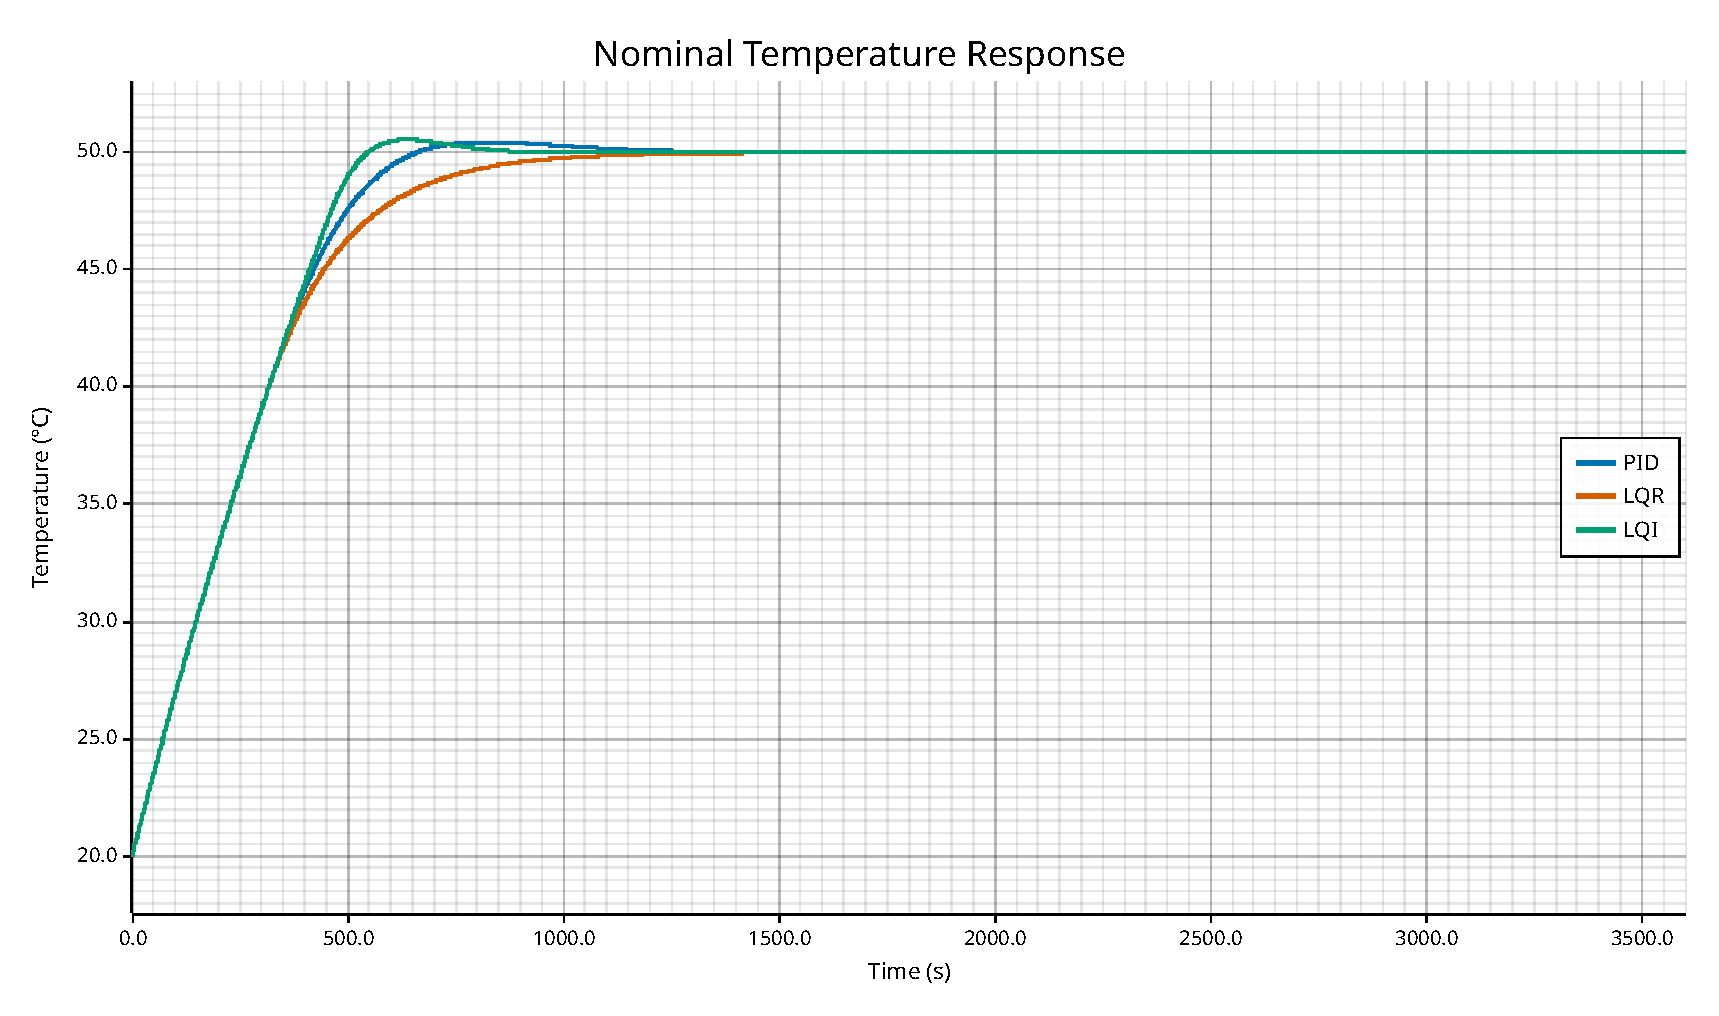
\includegraphics[width=\linewidth]{figures/nominal-temperature.pdf}\caption{기존 제어기의 공칭 추종.}\label{fig:nominal}\end{figure}
\begin{figure}[!htbp]\centering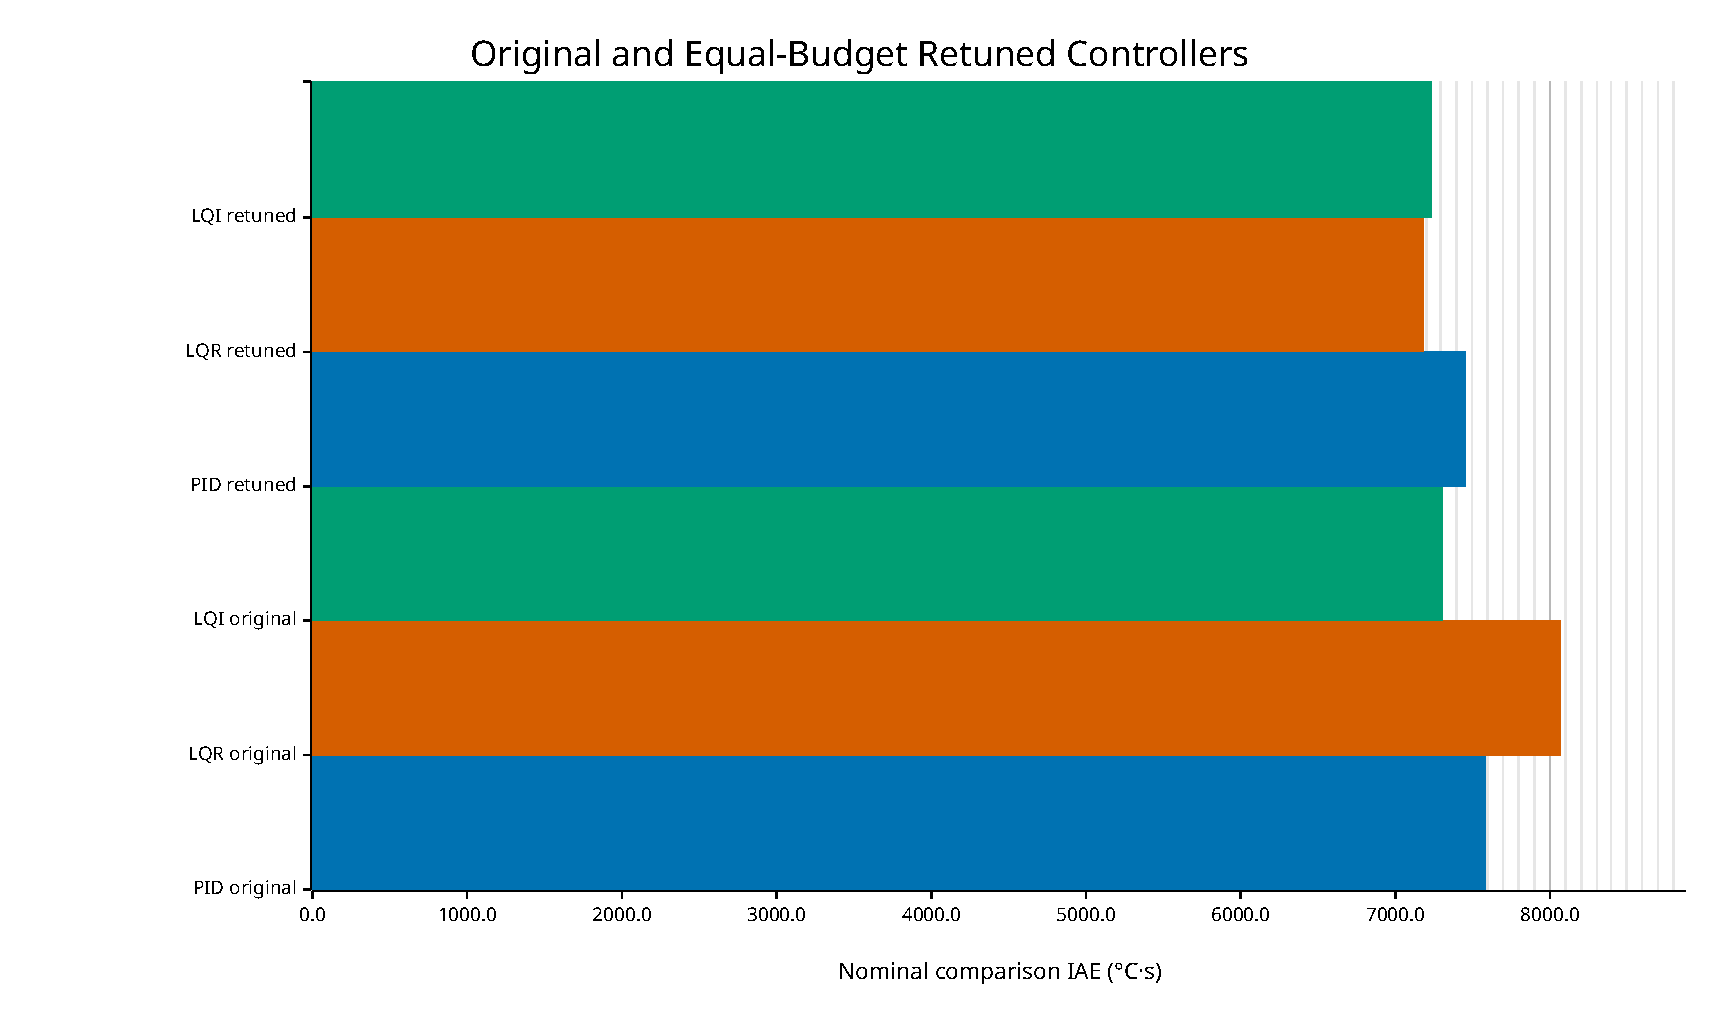
\includegraphics[width=\linewidth]{figures/original-vs-retuned.pdf}\caption{기존 및 동일 예산 재튜닝 공칭 IAE.}\label{fig:tuning}\end{figure}

\subsection{불확실성과 일정 부하 제거}
열용량 불확실성에 따른 기존 제어기의 RMSE 범위 변화는 PID, LQR, LQI 각각 1.824, 1.898, \SI{1.878}{\celsius}이고, 같은 백분율의 $UA$ 변화에서는 0.196, 0.276, \SI{0.203}{\celsius}이다. 시험 영역의 고정 시간 지표에서는 열용량의 영향이 더 크다(\cref{fig:uncertainty}).
\begin{figure*}[!t]\centering
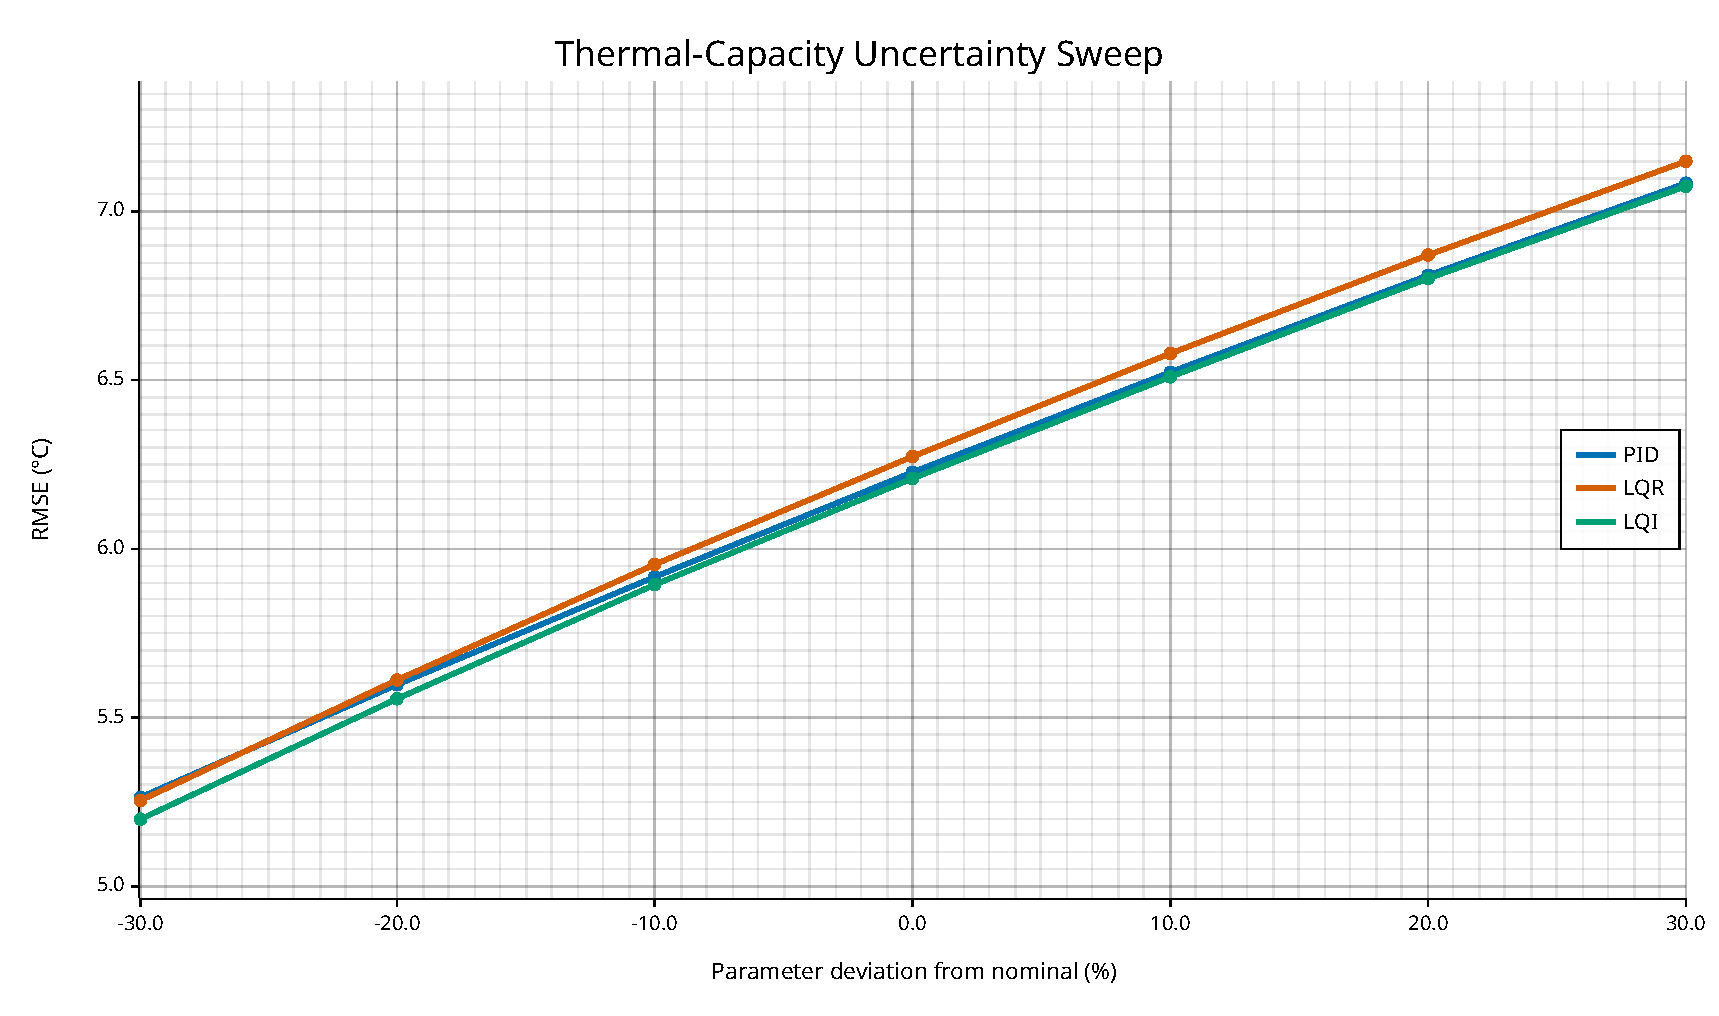
\includegraphics[width=.49\textwidth]{figures/capacity-uncertainty.pdf}\hfill
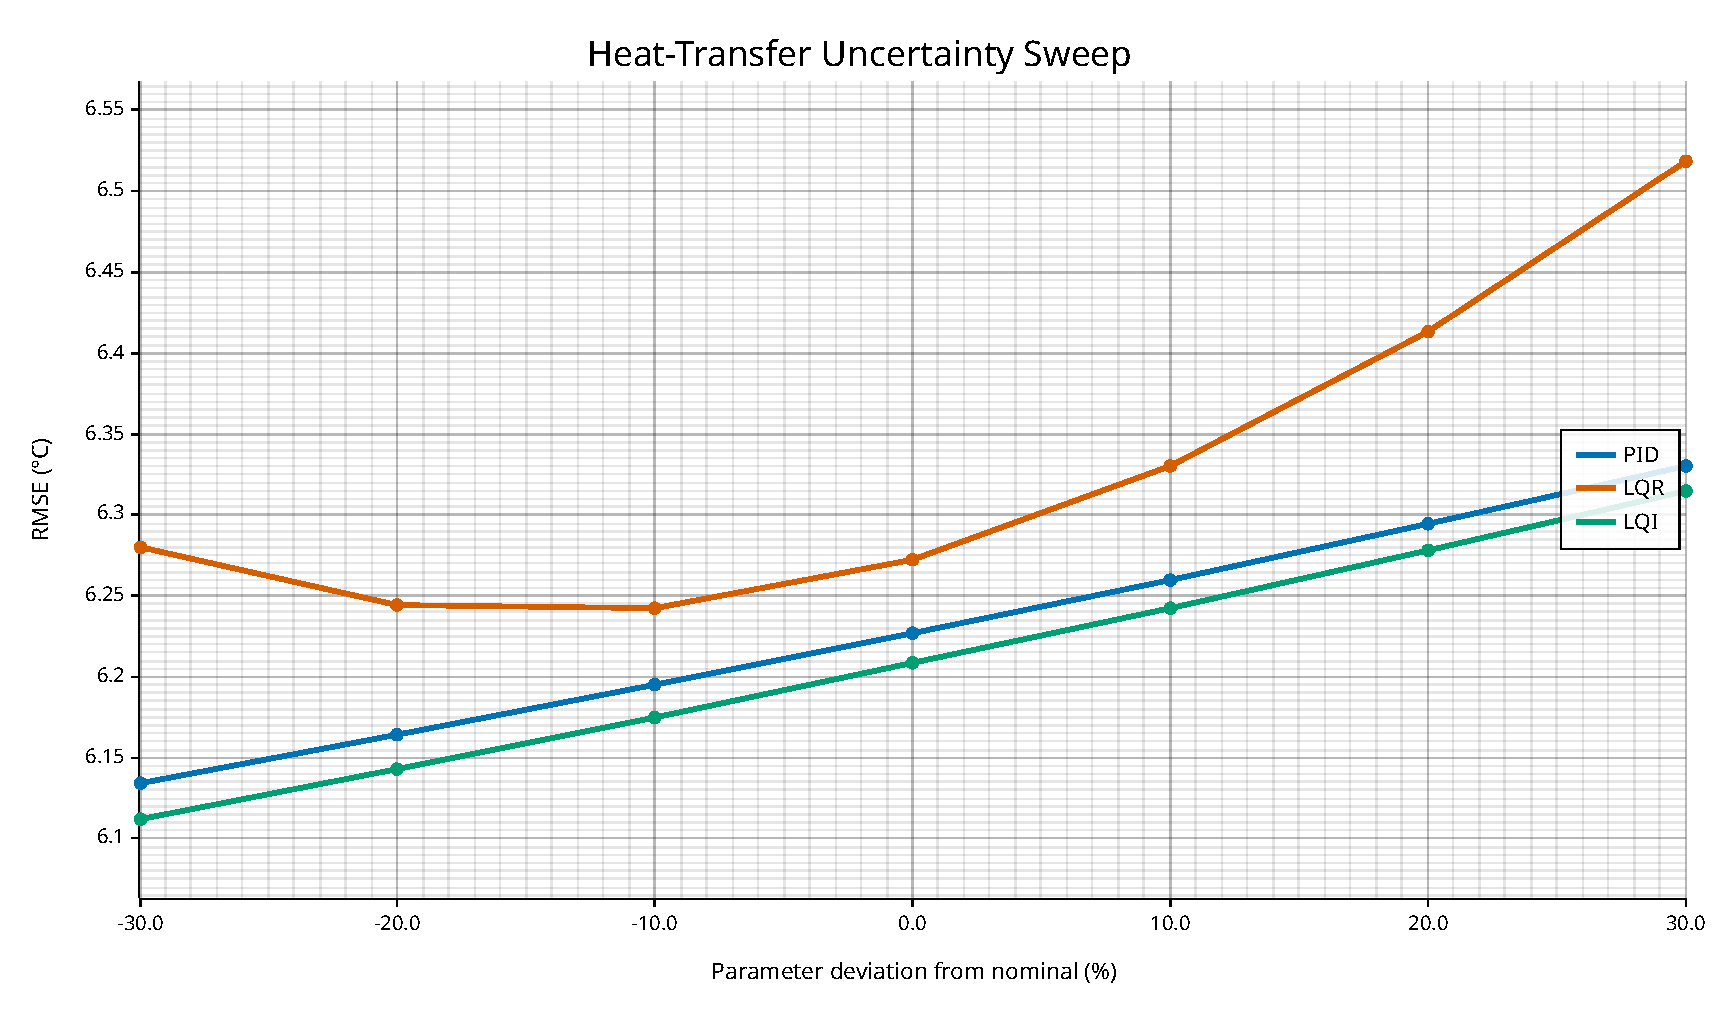
\includegraphics[width=.49\textwidth]{figures/heat-transfer-uncertainty.pdf}
\caption{열용량(왼쪽) 및 열전달(오른쪽) 불확실성에 대한 RMSE 민감도.}\label{fig:uncertainty}\end{figure*}

$-\SI{700}{W}$ 시험 부하 후 기존 제어기의 계단 이후 IAE는 PID 365.1, LQR 5006.4, LQI 118.9~$^\circ$C s이다. 말단 오차는 각각 약 0, 3.099, \SI{0}{\celsius}이다. 재튜닝 LQR은 훨씬 강한 비례 피드백으로 말단 오차를 \SI{0.079}{\celsius}까지 줄이지만 구조적 적분 제거 능력은 없다.
\begin{figure}[!htbp]\centering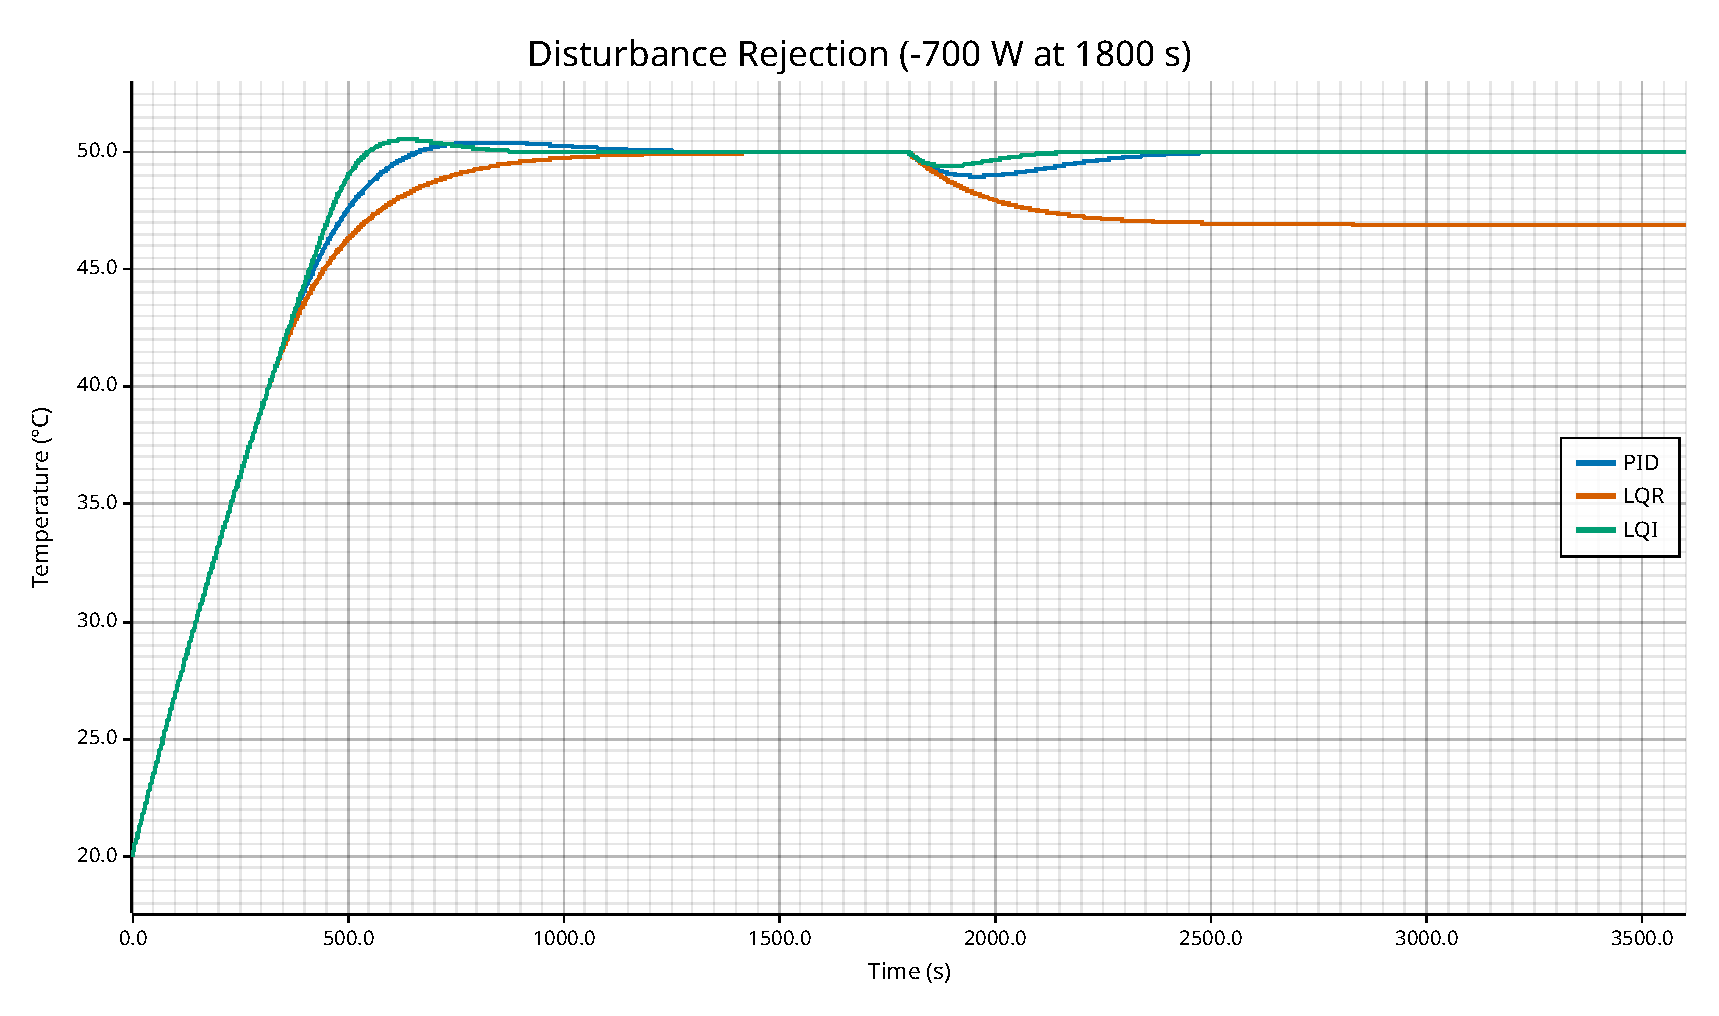
\includegraphics[width=\linewidth]{figures/disturbance-rejection.pdf}\caption{\SI{1800}{s}에서 $-\SI{700}{W}$ 부하에 대한 기존 제어기 응답.}\label{fig:disturbance}\end{figure}

\subsection{포화와 잡음}
수정된 기존 제한 액추에이터 IAE는 PID 25231.4, LQR 25268.5, LQI 25209.8~$^\circ$C s이다. 감사 전 LQR이 우세하다는 주장은 잘못된 안티와인드업 한계에서 비롯되었다. 재튜닝 제한 액추에이터 순위는 LQR(25200.3), LQI(25204.6), PID(25221.5)이며, 재튜닝 공칭 결과와 비교해 작은 순위 변화가 있다. 공통적으로 포화가 지배하는 과도응답에 비하면 차이는 매우 작다.
\begin{figure}[t]\centering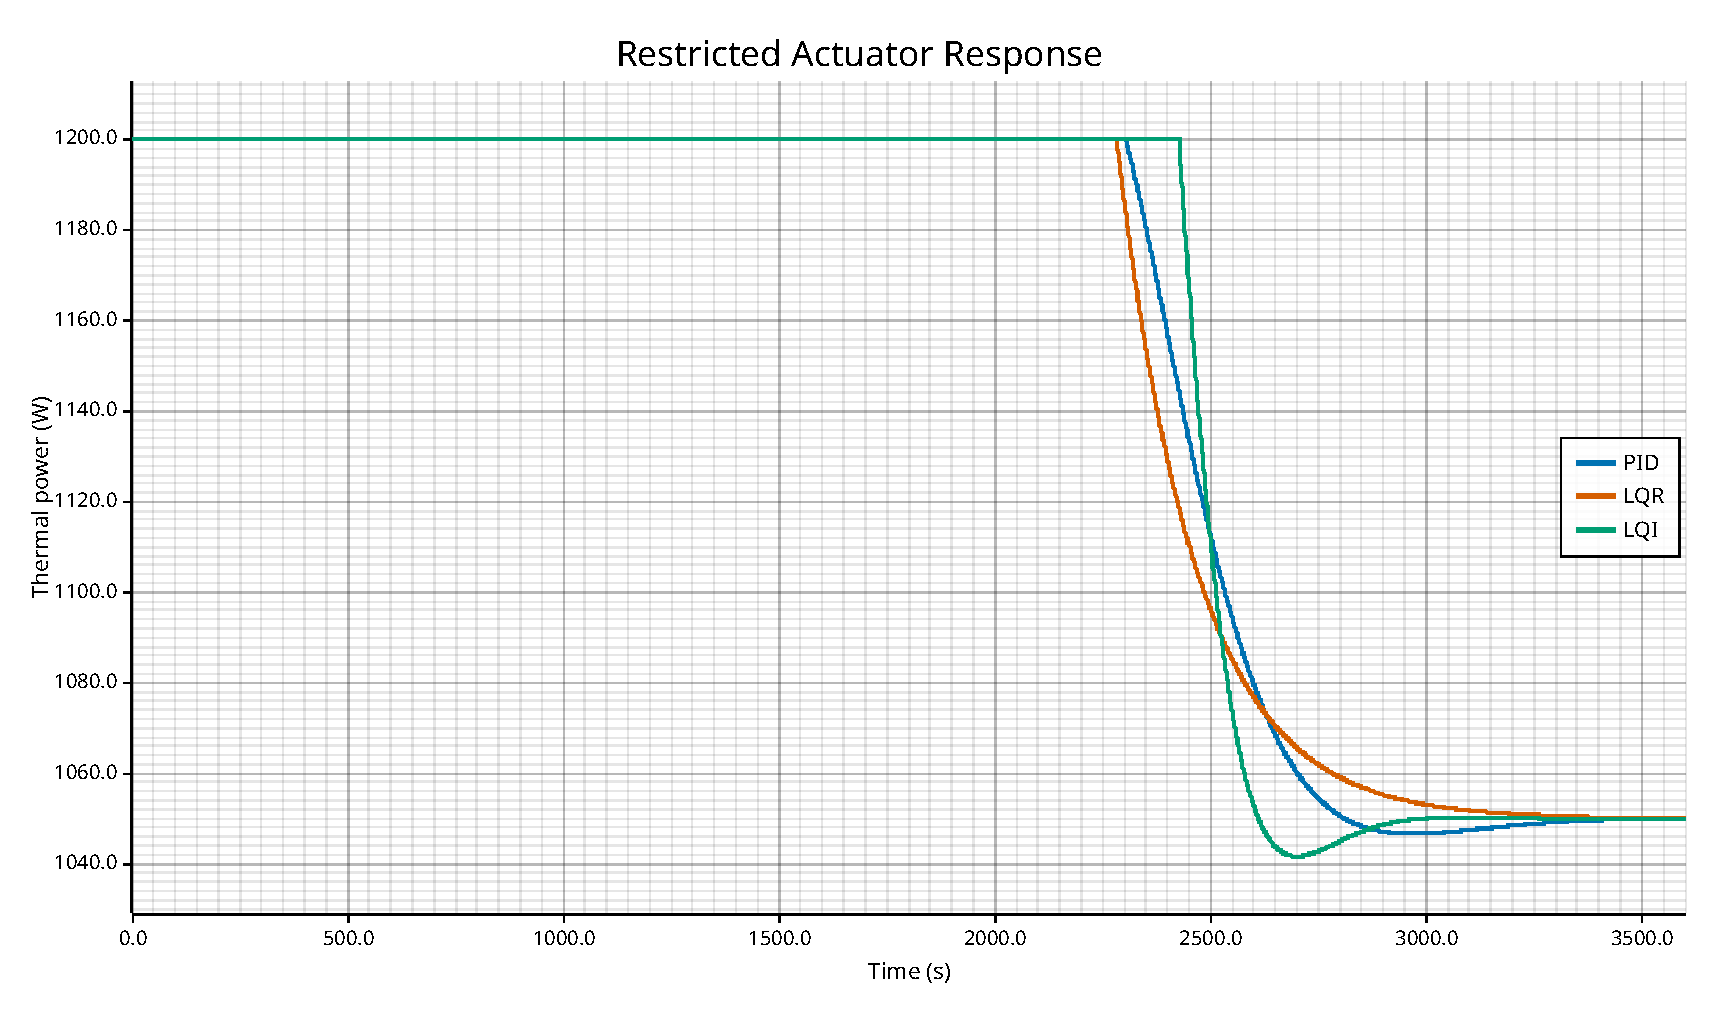
\includegraphics[width=\linewidth]{figures/actuator-saturation.pdf}\caption{제한된 한계에서 기존 제어기의 인가 동력.}\label{fig:saturation}\end{figure}

정상 구간에서 LQI와 PID의 짝지은 잡음 RMSE 차이는 \SI{0.004216}{\celsius}이다(95\% 신뢰구간 0.003978--0.004453, $d_z=3.52$). 반복 변동성이 매우 작아 표준화 효과크기는 크지만, 0.004도는 이 이상 공정에서 실용적으로 무시할 만하다. 잡음 크기나 스펙트럼이 달라지면 결론도 달라질 수 있으므로 센서 일반에 대한 주장은 하지 않는다.
\begin{figure}[t]\centering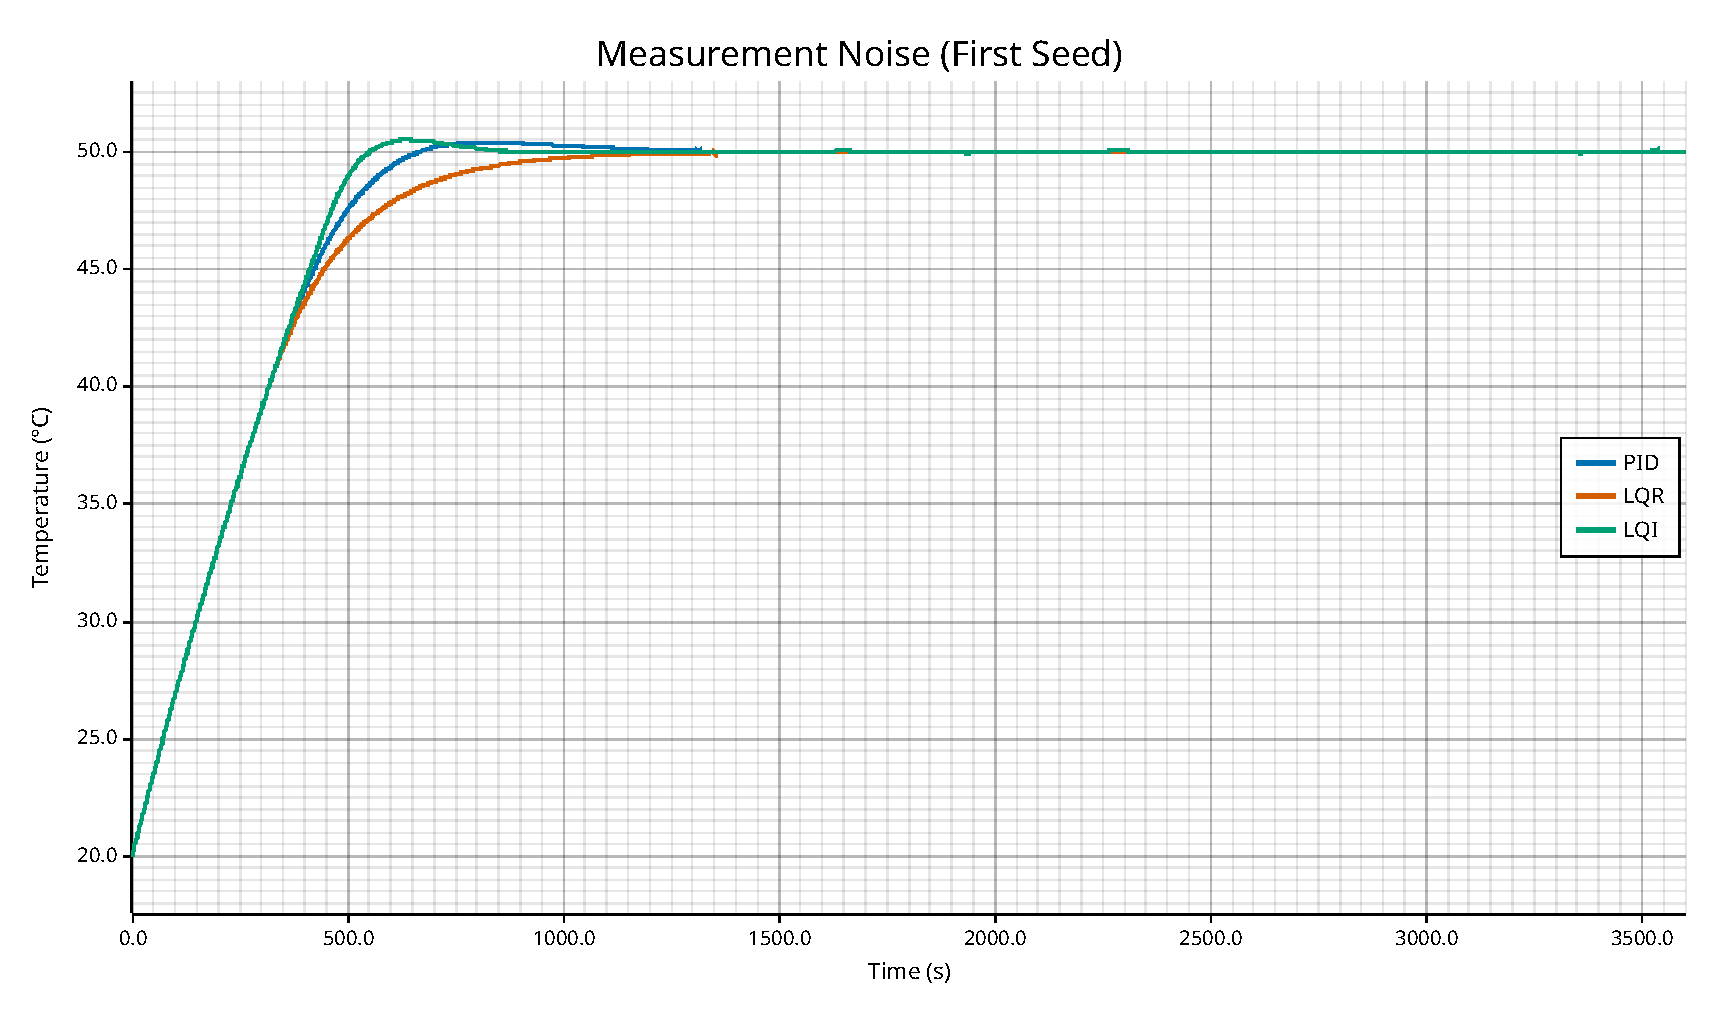
\includegraphics[width=\linewidth]{figures/measurement-noise.pdf}\caption{\SI{0.15}{\celsius} 측정 잡음의 한 짝지은 실현.}\label{fig:noise}\end{figure}

\subsection{모델에 포함되지 않은 센서 동특성}
지연 공정은 재튜닝 상충관계를 드러낸다(\cref{tab:fidelity,fig:fidelity}). 재튜닝 LQR IAE는 9345.2~$^\circ$C s로 증가하고 정착하지 않으며 2739~s 동안 포화된다. 기존 LQR IAE는 7804.1이다. PID와 LQI 변화는 훨씬 작다. 공격적인 공칭 튜닝은 단순 공정 성능을 높이지만 누락된 센싱 동특성에 대한 허용도를 낮춘다.
\begin{table}[!htbp]\centering\caption{Rust로 생성한 센서 지연 결과.}\label{tab:fidelity}\resizebox{\linewidth}{!}{\begin{tabular}{llrrr}\toprule
Design & Controller & IAE ($^\circ$C s) & RMSE ($^\circ$C) & Saturation (s) \\
\midrule
Original & PID & 7447.1 & 6.218 & 365 \\
Original & LQR & 7804.1 & 6.245 & 344 \\
Original & LQI & 7289.2 & 6.208 & 488 \\
Retuned & PID & 7364.1 & 6.215 & 395 \\
Retuned & LQR & 9345.2 & 6.252 & 2739 \\
Retuned & LQI & 7295.1 & 6.208 & 507 \\
\bottomrule\end{tabular}
}\end{table}
\begin{figure}[t]\centering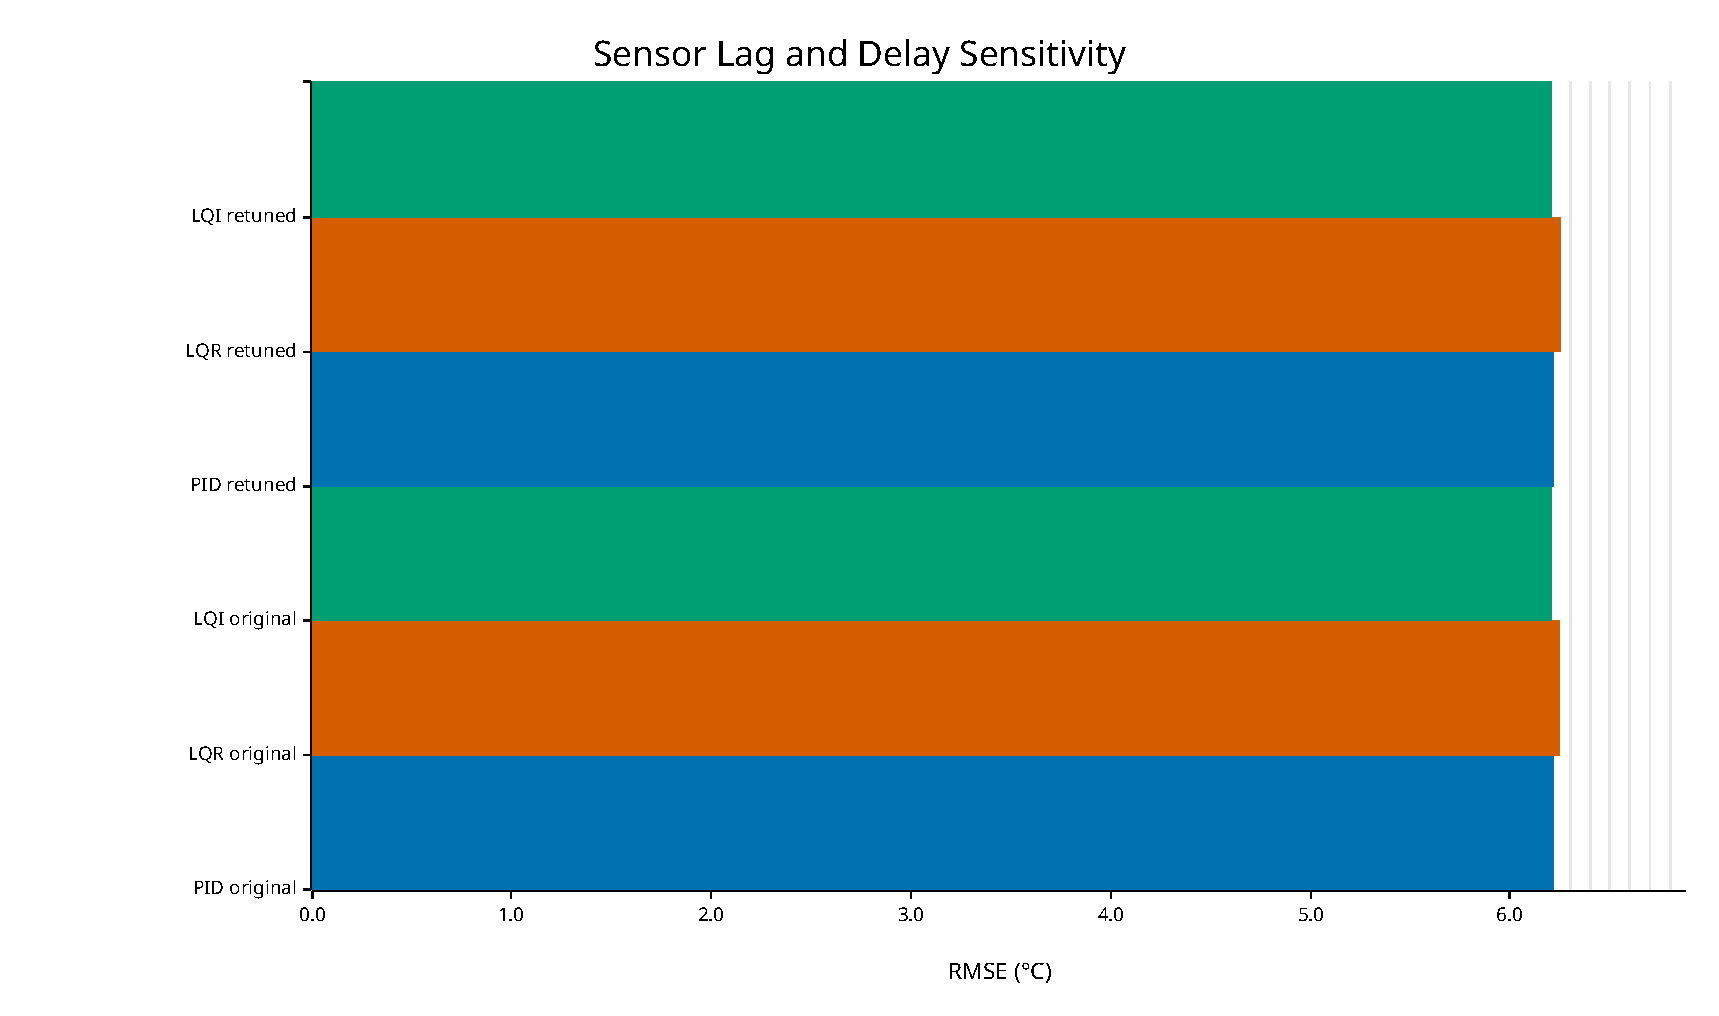
\includegraphics[width=\linewidth]{figures/higher-fidelity-summary.pdf}\caption{\SI{20}{s} 센서 지연과 \SI{10}{s} 순수 지연에서의 RMSE.}\label{fig:fidelity}\end{figure}
\FloatBarrier

\section{안정성 분석}\label{sec:stability}
아래 진술은 비포화·무잡음 선형 폐루프에 관한 것이며 포화 비선형 시뮬레이션으로 자동 확장되지 않는다.

LQR의 불확실 스칼라 특성방정식은
\begin{equation}
z-[A_d(C_{\rm th},UA)-B_d(C_{\rm th},UA)K]=0 \label{eq:lqrchar}
\end{equation}
이다. 연속 상자 $C_{\rm th}\in[0.7,1.3]C_0$, $UA\in[0.7,1.3]UA_0$에서 단조 지수 경계로 $A_d$와 $B_d$의 구간을 구한다. \cref{eq:lqrchar}의 자연 구간 평가는 단위원 여유 0.003961을 남겨 이 상자에서 기존 LQR을 형식적으로 인증한다.

LQI 폐루프 행렬은
\begin{equation}
F_{\rm LQI}=\begin{bmatrix}A_d-B_dK_x&-B_dK_z\\-h&1\end{bmatrix} \label{eq:lqimatrix}
\end{equation}
이다. 특성다항식 $z^2-tz+\delta$의 2차 Jury 조건은 $1-t+\delta>0$, $1+t+\delta>0$, $1-\delta>0$이다. $128^2$개의 덮개 부분 상자에서 바깥쪽으로 보수적인 구간 평가를 수행한 최소 여유는 각각 $3.19\times10^{-5}$, 3.95, 0.0137이다. 모두 양수이므로 연속 상자 전체에서 기존 LQI 안정성이 인증된다. 세분화는 의존성 과대평가만 줄이며 점을 누락하지 않는다.

구현된 PID는 적분 상태, 필터 미분 상태, 이전 측정값 때문에 4차 선형 실현을 갖는다. 특성방정식은 $\det(zI-F_{\rm PID})=0$이며 $F_{\rm PID}$는 이산 갱신식에서 직접 생성한다. 61×61 격자의 스펙트럼 반경은 0.992397--0.995996이지만 계수 의존성 때문에 현재 구간 계산으로 전체 상자를 증명하지 못했다. 따라서 PID의 형식적 강인 안정성은 미증명 상태이다.
\begin{table}[!htbp]\centering\caption{형식적 및 격자 기반 안정성 근거.}\label{tab:stability}\resizebox{\linewidth}{!}{\begin{tabular}{lcc}\toprule
Controller & Formal interval result & Grid radius range \\
\midrule
PID & Unproven & 0.992397--0.995996 \\
LQR & Certified (margin 0.003961) & 0.991930--0.996039 \\
LQI & Certified (min. Jury margin 0.000032) & 0.986843--0.993128 \\
\bottomrule\end{tabular}
}\end{table}
\begin{figure}[t]\centering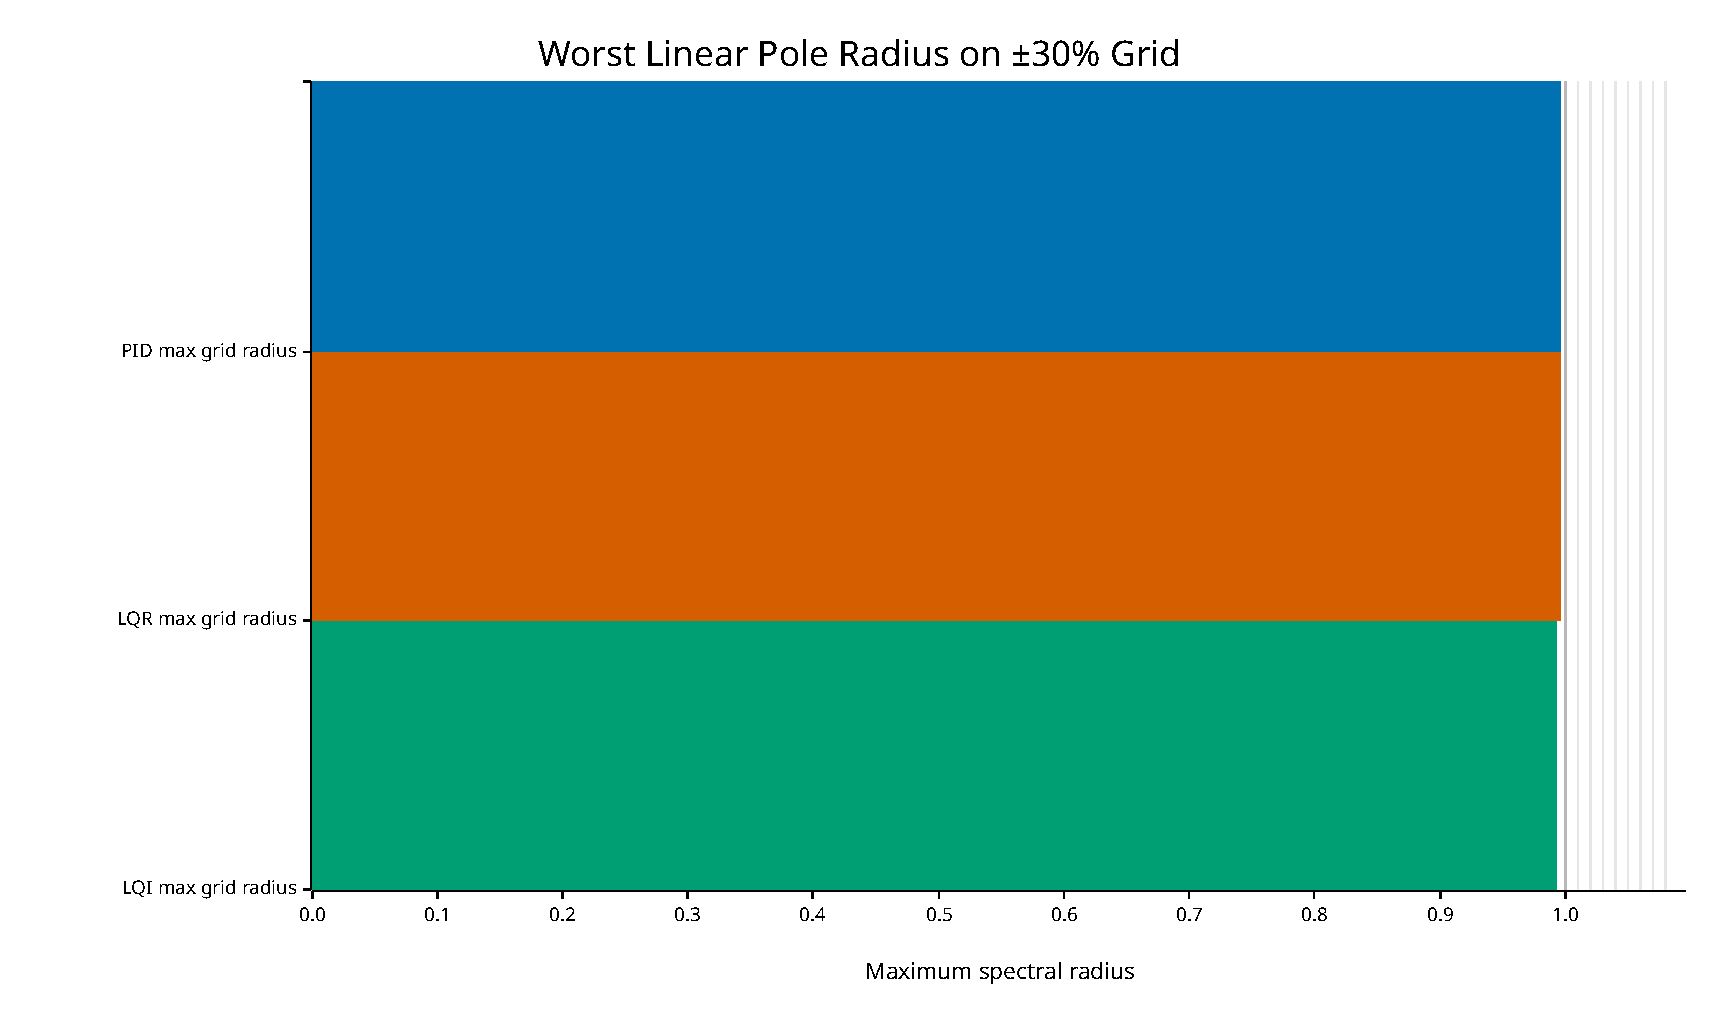
\includegraphics[width=\linewidth]{figures/stability-domain-summary.pdf}\caption{정수 불확실성 격자에서의 최악 스펙트럼 반경. 구간 증명이 아니라 보조 수치 근거이다.}\label{fig:stability}\end{figure}
\FloatBarrier

\section{논의}\label{sec:discussion}
수정된 근거는 제어기 구조와 튜닝을 구분한다. 기존 LQI는 공칭 추종과 부하 제거에서 우세하고, 동일 예산 튜닝에서는 매우 높은 피드백 권한을 택한 LQR이 공칭 비교에서 우세하다. 이 이점은 조건부이다. 센싱 지연은 지속적인 포화를 유발하고 공칭 이점을 제거한다. 적분 동작은 실현 가능한 일정 열부하를 안정적으로 제거하지만 LQI가 잡음, 포화, 누락 동특성에서 항상 최선은 아니다.

안티와인드업 수정은 과학적으로 중요하다. 수정 전에는 공정이 더 좁은 한계를 사용하는 동안 PID와 LQI가 공칭 한계에 대해 적분했다. 수정 결과는 제한 액추에이터에서 기존 LQR이 가장 좋다는 이전 가설을 지지하지 않는다. 재튜닝 이득에서는 LQR의 제한 IAE가 근소하게 가장 작지만 차이는 실용적으로 작고 모든 제어기에서 포화가 지배적이다.

같은 후보 수와 시나리오는 공정성을 높이지만 최적화 난이도를 같게 하지는 않는다. LQR은 두 가중치, PID와 LQI는 세 매개변수를 탐색하고 매개변수-응답 사상도 다르다. 따라서 결과는 통제된 유한 예산 비교로 보는 것이 적절하다. 독립 가우시안 실현의 통계적 신뢰도 역시 몬테카를로 정밀도를 나타낼 뿐 실제 센서 물리나 공정 매개변수 불확실성을 뜻하지 않는다.

화학적 역할은 의도적으로 제한했다. 모델은 비반응성 액체의 용액 열용량, 열전달, 열평형을 표현한다. 반응기 동역학, 농도, 산업 장비, 실험실 검증을 주장하지 않는다.

\section{한계}
매개변수는 예시값이며 물리 측정값이 없다. 완전혼합, 일정 물성, 선형 열손실, 순간 구동, 가우시안 백색 센서 잡음은 단순화 가정이다. 보조 모델은 센서 지연을 추가하지만 검증된 산업 모델이 아니다. LQR과 LQI만 연속 상자에 대한 형식적 인증을 갖고 PID는 조밀한 격자 근거만 갖는다. 포화 폐루프의 안정성은 증명하지 않았다. 튜닝 예산은 탐색 복잡도가 아니라 평가 횟수만 동일하며 공칭 비교는 훈련 시나리오와 겹친다. 신뢰구간은 한 잡음 분포 아래의 독립 의사난수 스트림을 가정한다. 따라서 본 연구는 조건부 시뮬레이션 결론만을 뒷받침한다.

\section{결론}
감사된 시뮬레이션 결과, 제어기 순위는 목적함수, 모델 불일치, 누락 동특성에 따라 달라졌다. 동일 예산 튜닝은 공칭 순위를 LQI--PID--LQR에서 LQR--LQI--PID로 바꾸지만 작은 센서 지연은 튜닝 LQR의 이점을 제거한다. 적분 동작의 가장 명확한 이점은 일정 부하 제거이다. 고정 시간 RMSE에는 같은 백분율의 열전달 불확실성보다 열용량 불확실성이 더 큰 영향을 미쳤다. 포화 처리 수정으로 기존 부정적 결과가 무효화되었고 잡음 차이는 통계적으로 명확하지만 실용적으로 작다. 구간 분석은 선언한 연속 매개변수 상자에서 기존 LQR과 LQI의 비포화 강인 안정성을 증명하지만, PID와 모든 포화 폐루프의 근거는 명시적으로 제한된다. 저장소는 새로운 제어 알고리즘이나 실제 공정 검증이 아니라 재현 가능한 연구 결과를 제공한다. 향후 연구는 물리 실험을 요구하지 않고 구간 분석, 지연 강인 튜닝, 유색 잡음, 고차 열 네트워크로 확장할 수 있다.

\section*{재현성 선언}
실행 가능한 모든 연구 코드는 Rust로 작성되었다. 저장소는 Rust 1.100.0과 의존성 버전을 고정하고, 설정 및 시드를 기록하며, 계산 결과에서 표와 벡터 그림을 생성하고, 제공된 템플릿 절차로 논문을 다시 빌드한다. 전체 연구는 \texttt{cargo run --release -- run-all} 실행 후 \texttt{paper/}에서 \texttt{make}로 재현한다.

\printbibliography[title={참고문헌}]
\end{document}
